% --------------------------------------------------------------
% This is all preamble stuff that you don't have to worry about.
% Head down to where it says "Start here"
% --------------------------------------------------------------

\documentclass[12pt]{article}

\usepackage[margin=1in]{geometry}
\usepackage{amsmath,amsthm,amssymb}
\usepackage{graphicx} %This allows to include eps figures
\usepackage{subcaption}
\usepackage[section]{placeins}
\usepackage{layout}
\usepackage{etoolbox}
\usepackage{mathabx}
\usepackage{animate}
\usepackage{array}
% This is to include code
\usepackage{listings}
\usepackage{xcolor}
\usepackage{fontenc}
\usepackage{kantlipsum}
\usepackage[breakable, theorems, skins]{tcolorbox}

\definecolor{dkgreen}{rgb}{0,0.6,0}
\definecolor{gray}{rgb}{0.5,0.5,0.5}
\definecolor{mauve}{rgb}{0.58,0,0.82}
% set the default code style
\lstset{
    frame=tb, % draw a frame at the top and bottom of the code block
    tabsize=4, % tab space width
    showstringspaces=false, % don't mark spaces in strings
    numbers=left, % display line numbers on the left
    commentstyle=\color{green}, % comment color
    keywordstyle=\color{blue}, % keyword color
    stringstyle=\color{red} % string color
}
\lstdefinestyle{Python}{
    language        = Python,
    basicstyle      = \ttfamily,
    keywordstyle    = \color{blue},
    keywordstyle    = [2] \color{teal}, % just to check that it works
    stringstyle     = \color{green},
    commentstyle    = \color{red}\ttfamily
}
\lstdefinestyle{C++}{
    float=h!, 
    frame=single, 
    language={[Visual]C++}, 
    numbers=left, 
    numberstyle=\tiny, 
    tabsize=2, 
    breaklines=true
}

\newenvironment{conditions}
  {\par\vspace{\abovedisplayskip}\noindent\begin{tabular}{>{$}l<{$} @{${}={}$} l}}
  {\end{tabular}\par\vspace{\belowdisplayskip}}

\newcommand{\N}{\mathbb{N}}
\newcommand{\Z}{\mathbb{Z}}

\newenvironment{theorem}[2][Theorem]{\begin{trivlist}
\item[\hskip \labelsep {\bfseries #1}\hskip \labelsep {\bfseries #2.}]}{\end{trivlist}}
\newenvironment{lemma}[2][Lemma]{\begin{trivlist}
\item[\hskip \labelsep {\bfseries #1}\hskip \labelsep {\bfseries #2.}]}{\end{trivlist}}
\newenvironment{exercise}[2][Exercise]{\begin{trivlist}
\item[\hskip \labelsep {\bfseries #1}\hskip \labelsep {\bfseries #2.}]}{\end{trivlist}}
\newenvironment{reflection}[2][Reflection]{\begin{trivlist}
\item[\hskip \labelsep {\bfseries #1}\hskip \labelsep {\bfseries #2.}]}{\end{trivlist}}
\newenvironment{proposition}[2][Proposition]{\begin{trivlist}
\item[\hskip \labelsep {\bfseries #1}\hskip \labelsep {\bfseries #2.}]}{\end{trivlist}}
\newenvironment{corollary}[2][Corollary]{\begin{trivlist}
\item[\hskip \labelsep {\bfseries #1}\hskip \labelsep {\bfseries #2.}]}{\end{trivlist}}

\DeclareRobustCommand{\important}[2][gray!20]{%
\begin{tcolorbox}[   %% Adjust the following parameters at will.
  breakable,
  left=0pt,
  right=0pt,
  top=0pt,
  bottom=0pt,
  colback=#1,
  colframe=#1,
  width=\dimexpr\textwidth\relax, 
  enlarge left by=0mm,
  boxsep=5pt,
  arc=0pt,outer arc=0pt,
  ]
  #2
\end{tcolorbox}
}


\begin{document}

% --------------------------------------------------------------
%                         Start here
% --------------------------------------------------------------

%\renewcommand{\qedsymbol}{\filledbox}

\title{Summary I}%replace X with the appropriate number
\author{Nalet Meinen\\ %replace with your name
C++ Programming I
}


 


\maketitle


\begin{figure}[!htb]
  \centering
  \vspace*{4cm}
  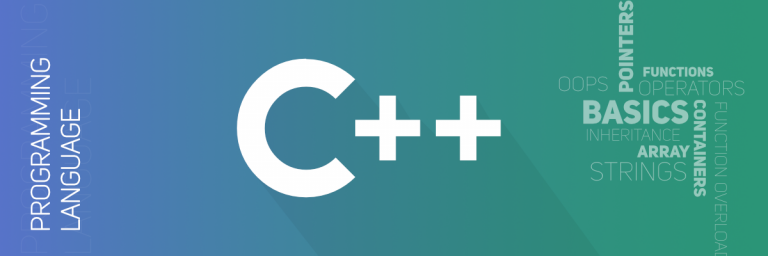
\includegraphics[width=1.0\linewidth]{pics/title}
\end{figure}

  \pagebreak

\tableofcontents
\pagebreak


\section{Basics}
\subsection{Variables}

\begin{lstlisting}[caption={Declaration, Initialisation and Definition}, style=C++]
//Declaration
int x; //of variable int
intgetValue(); //of function prototype
//Definition
int x; //same as declaration
int getValue(){ /*Definition*/ }// without ';'
//Initialisation is optional, but it's
//often a good programming practice
int x=42;//refers to the "assignment" of a value
//initialization does not mean much for functions
}
\end{lstlisting}
\begin{itemize}
\item The variable type attribute tells the compiler the nature of data the
      variable can store, and the compiler reserves the necessary space for it
\item The variable name is a friendly replacement for the address in the
      memory
\item Use camelCase naming convention for variables
\item Naming conventions differs for objects, functions etc.
\end{itemize}

\important[red!20!white]{
Naming variables appropriately is important for writing good,
understandable, and maintainable code!
}

\section{Functions}
\section{Pointers and References}
\section{Fundamentals of Object Oriented C++ Programming}
\section{Classes and Objects}

% \pagebreak
% \begin{thebibliography}{9}

  
%   \bibitem{natural frequencies} 
%   Barry J. Goodno, James McGere
%   \textit{Mechanics of Materials (2018)}. (English)  

%   \bibitem{latexcompanion} 
%   Michel Goossens, Frank Mittelbach, and Alexander Samarin. 
%   \textit{The \LaTeX\ Companion}. 
%   Addison-Wesley, Reading, Massachusetts, 1993.
% \end{thebibliography}


\end{document}